
\section{metabolism.xml}

The metabolism file is strongly inspired by SBML.\@
More precisely, it can be seen as a subpart of an SBML file.
It is used to define compartments, metabolites and reactions.

\subsection{Rationale}

metabolism.xml contains the most basic bricks of an RBA model.
In our effort to define a minimal structure that contains an RBA model,
we decided to start with an SBML structure and strip it down to elements that
are essential to RBA.

metabolism.xml defines the structure of the metabolic network:
simple chemical species (metabolites) that flow between compartments through
transport reactions or transformed into other simple chemical species that
will be available as building blocks for more complex molecules.

The description is entirely static: input fluxes are defined
through the medium and parameters.xml, output fluxes are
defined by targets.xml, the dynamics of internal fluxes is
defined in enzymes.xml.

\subsection{RBAMetabolism}
\label{sec:rba_metabolism}

The outermost part of the metabolism file is an instance of class
\rbametabolism, shown in Figure~\ref{fig:metabolism_doc}.

\begin{figure}
  \centering
  \includegraphics[scale=0.8]{figures/metabolism_doc}
  \caption{XML structure of metabolism document.}
\label{fig:metabolism_doc}
\end{figure}

Currently, \rbametabolism{} has no simple attributes.
It includes exactly one instance of each \textbf{ListOf} container class.
All \textbf{ListOf} classes do not have own attributes,
they are merely used to organize a list of instances from another class.
This organization was inspired by SBML.\@


\subsection{Compartment}
\label{sec:compartment}

The \compartment{} class is used to list existing cell compartments.

\paragraph{The \textit{id} attribute}
The \textbf{id} attribute is a string defining the identifier of a compartment.
Every compartment should have a different id.


\subsection{Species}
\label{sec:species}

The \species{} class is used to define \emph{metabolic} species.

\paragraph{The \textit{id} attribute}
The \textbf{id} attribute is a string defining the identifier of a metabolite.

\paragraph{The \textit{boundaryCondition} attribute}
The \textbf{boundaryCondition} attribute is a boolean.
If the attribute is set to true, the metabolite is considered to be at
a constant concentration.
In other words, it is not affected by reactions.
This is typical for metabolites in the external medium.


\subsection{Reaction}
\label{sec:reaction}

The \reaction{} class is used to define metabolic reactions
(Fig.~\ref{fig:metabolism_reaction}).
Reactants and products are defined using a \textbf{ListOfSpeciesReferences}.

\begin{figure}
  \centering
  \includegraphics[scale=0.8]{figures/metabolism_reaction}
  \caption{Class storing metabolic reactions.}
\label{fig:metabolism_reaction}
\end{figure}

\paragraph{The \textit{id} attribute}
The \textbf{id} attribute is a string defining the identifier of a reaction.

\paragraph{The \textit{reversible} attribute}
The \textbf{reversible} attribute is a boolean.
If the attribute is set to true, the reaction can occur in both directions.
If the attribute is set to false, only the forward reaction can occur.


\subsection{SpeciesReference}
\label{sec:species_reference}

The \speciesreference{} class is used to refer to a metabolic \species{}
and associate with it a stoichiometry (Fig.~\ref{fig:metabolism_reaction}).

\paragraph{The \textit{species} attribute}
The \textbf{species} attribute must match the identifier of a \species{}.

\paragraph{The \textit{stoichiometry} attribute}
The \textbf{stoichiometry} is a positive real number.
It repensents the stoichiometry of a \species{} in a given context
(typically a \reaction).

\subsection{Examples}

Figure~\ref{fig:metabolism_ex_1} shows a very simple example with 2 compartments,
4 metabolites and 3 reactions.
In this example, we tagged \texttt{M\_carbon\_source\_e} with \texttt{boundary\_condition="true"},
implying that it is an external metabolite whose concentration is known and set through the
medium in medium.tsv.
Boundary metabolites are essential in the model, as they define input fluxes in the model.

\begin{figure}
  \includegraphics[scale=0.6]{figures/metabolism_ex_1}
  \caption{metabolism.xml from the minimal model with 2 compartments,
  4 metabolites and 3 reactions.}
\label{fig:metabolism_ex_1}
\end{figure}

Note that the description of the metabolic network ends with the protein precursor.
Proteins \emph{should not} be defined in metabolism.xml.
Their composition is described in proteins.xml, while their assembly is described in processes.xml.
